\documentclass[a4paper,11pt]{article}
%\usepackage[T1]{fontenc}

%\setlength{\textwidth}{20cm}
%\setlength{\marginparwidth}{0cm}
%\setlength{\voffset}{0cm}
\usepackage[utf8]{inputenc}
\usepackage[francais]{babel}
\usepackage{amsmath}
\usepackage{graphicx}
\usepackage{listings}
\usepackage{color}
\usepackage{url}
%==== to fix locations of figures and tables
\usepackage{float}
\usepackage{placeins}

\usepackage{subfigure}

\lstset{
language=VHDL,
basicstyle=\small\sffamily,
%numbers=left,
%numberstyle=\tiny,
%frame=tb,
columns=fullflexible,
showstringspaces=false
}
%\special{papersize=210mm,297mm}

\title{{\Huge Electronique numérique}\\Initiation à VHDL (3/3)\\Synthèse sur FPGA}
%\title{TD1}
\date{}

\begin{document}
\maketitle

% Ce BE d'Electronique nous permet d'expérimenter quelques aspects non traités jusqu'ici :
% \begin{itemize}
%   \item Manipulations binaires en Python
%   \item Synthèse sur FPGA
%   \item Communication entre un ordinateur et un FPGA
% \end{itemize}

Ce BE d'Electronique vise à concevoir un circuit concret et le synthétiser sur FPGA.

\paragraph{Remarque 1 :} Il n'est pas possible de vous mettre à disposition un tel FPGA par personne, ni même
par binôme (plusieurs groupes en parallèle). Vous pourrez accéder aux cartes à tour de rôle. Ces objets
sont \underline{fragiles} et \underline{coûteux}. \textbf{Merci d'en prendre le plus grand soin} : notamment le cable
USB doit être manipulé avec précaution.

\paragraph{Remarque 2 :} Lancer la commande suivante afin de bénéficier des logiciels d'Electronique.
\begin{lstlisting}{language=bash}
 $ module load electronique
\end{lstlisting}

%\section{Manipulations binaires en Python}

\section{Synthèse sur FPGA : serrure numérique}
\paragraph{Spécifications}
Nous cherchons à réaliser le système numérique suivant, dont les spécifications peuvent se résumer ainsi :
une porte est sécurisée par un code d'accès. Si le code tapé est correct,
une diode clignote pendant 5 secondes, la porte s'ouvre et se referme en 5 secondes, et l'accès est alors à nouveau protégé.\\

Voici quelques éléments techniques :

\paragraph{Carte et FPGA}
Le clavier est connecté à une carte Nexys4DDR de la société Digilent (fig \ref{nexys4ddr}).
\begin{figure}
  \centering
  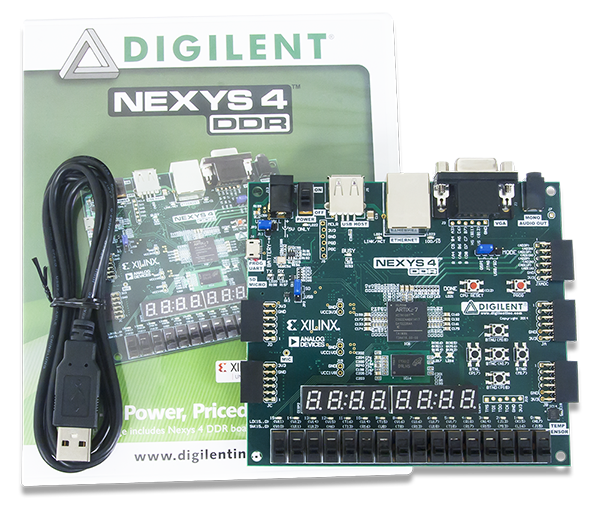
\includegraphics[width=5cm]{./figures/nexys4ddr.png}
  \label{nexys4ddr}
  \caption{Carte Digilent Nexys4DDR avec Xilinx Artix-7}
\end{figure}

Cette carte embarque une FPGA Artix7 de la société Xilinx \footnote{Inventeur des FPGA, et leader mondial avec Intel}.
Les ports d'entrées/sorties (ou "pattes") du FPGA ont été soudés par Digilent : ils sont connectés 1 par 1 vers des connecteurs d'extensions comme les PMOD que nous allons utiliser, mais également des
composants discrets présents sur cette même carte :
boutons, LEDs, interrupteurs, VGA, micro, mémoire externe, accéléromètre,
 micro, capteur de température, carte SD, ethernet ! Il n'est évidemment pas possible de modifier (ou "reconfigurer") ces connexions.
Votre code VHDL sera synthétisé au sein du FPGA, à l'inverse intégralement \textbf{reconfigurable}.

\paragraph{Synthèse et chargement sur FPGA}

Nous procéderons par \textit{script de synthèse}, que l'on peut lancer directement
en ligne de commande \footnote{Pour information, ce script est écrit dans le langage TCL, langage de script très utilisé pour commander des logiciels, y compris en dehors de l'Electronique.}.
Ce script permet donc de passer du VHDL à un circuit (netlist) et génère au final un fichier appelé \textit{bitstream}, qui permet de configurer le FPGA avec vos portes logiques.
Il faut par ailleurs indiquer au préalable une \textit{correspondance} (ou "mapping") entre votre entité VHDL (vos entrées/sorties nommées)
et les pattes physiques du FPGA. Cette mise en correspondance se fait dans un \textit{fichier de contraintes} dont l'extension est {\it .xdc}. Enfin, le bitstream sera chargé sur FPGA à l'aide d'une autre commande, donnée par Digilent.

Afin de simplifier la manipulation, ces différents éléments sont donnés sous Moodle.
\begin{itemize}
  \item Entité VHDL du circuit à réaliser, ainsi qu'une architecture partiellement concue (vous devrez y instancier quelques composants, discutés par la suite).
  \item Script de synthèse (script.tcl).
  \item Fichier de contraintes : Nexys4DDR.xdc
\end{itemize}

Le fait de vous donner cette entité vous affranchi d'écrire vous-mêmes le fichier xdc, ainsi que le script de synthèse.\\

\paragraph{Commandes Linux}

La procédure de mise au point se fera de la manière suivante :
\begin{itemize}
  \item Analyse syntaxique avec GHDL :
  \begin{lstlisting}{language=bash}
    $ ghdl -a nom.vhd
  \end{lstlisting}
  \item Synthèse FPGA avec la commande :
  \begin{lstlisting}{language=bash}
    $ vivado -mode tcl -source script.tcl
  \end{lstlisting}
  \item Chargement sur FPGA du bitstream "top.bit" généré par la commande précédente :
  \begin{lstlisting}{language=bash}
    $ djtgcfg prog -d Nexys4DDR -i 0 -f SYNTH_OUTPUTS/top.bit
  \end{lstlisting}
\end{itemize}


\section{Principe de fonctionnement du clavier}
Le clavier 16 boutons est un matériel très frustre, comme on peut l'observer sur la figure \ref{clavier} :
outre les boutons, seules des resistances de pullup sont nécessaires à sa constitution \footnote{Tout nous porte à penser que les touches sont aidées d'un mécanisme
d'{\it anti-rebond} \url{http://hades.mech.northwestern.edu/index.php/Switch_Debouncing}.}.

\begin{figure}
  \centering
  \begin{subfigure}
    \centering
    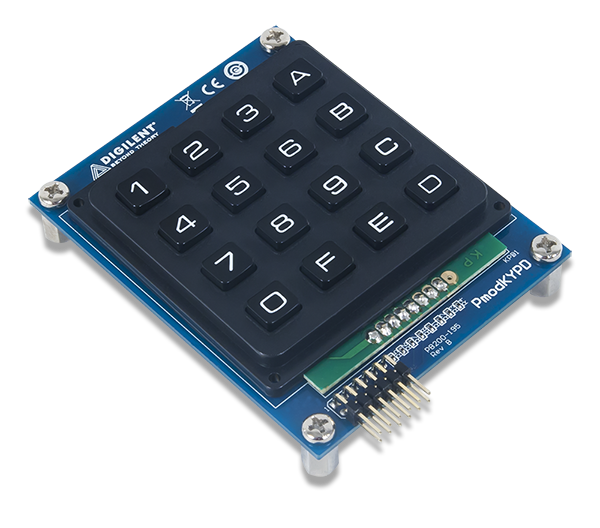
\includegraphics[width=4cm]{./figures/keyboard_1.png}
  \end{subfigure}%
  \begin{subfigure}
    \centering
    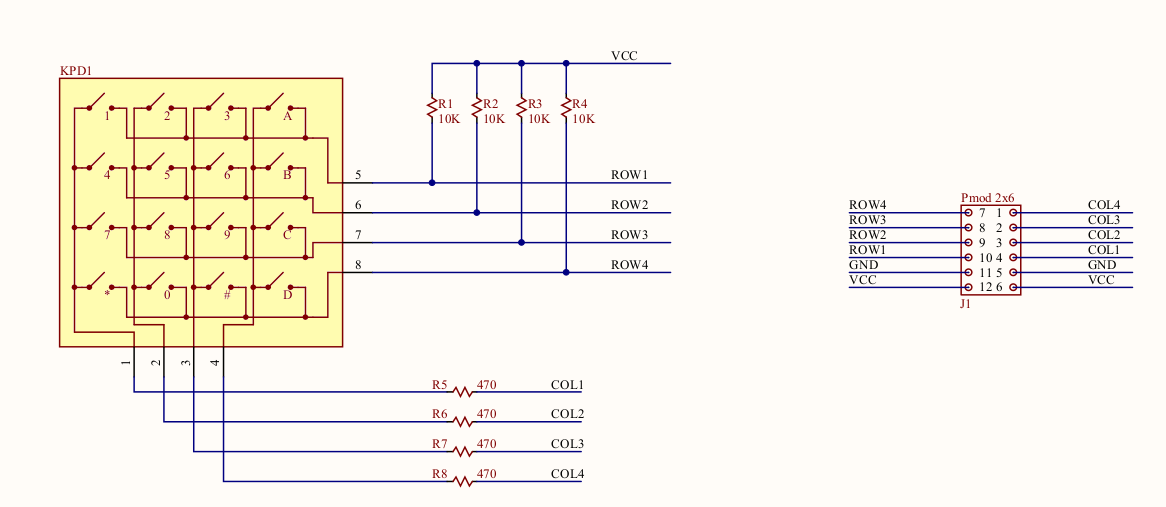
\includegraphics[width=10cm]{./figures/keyboard_2.png}
  \end{subfigure}
  \caption{Clavier 16 touches}
  \label{clavier}
\end{figure}

Le principe de fonctionnement est le suivant : sans appui sur un bouton, les résistances de pull-up
conduisent les sorties "row" à 3.3 v (le 1 logique sur ce FPGA). Lorsqu'on appuie sur un bouton, les tensions des sorties row
dépendent des tensions appliquées sur les entrées "column". Pour détecter le bouton sur lequel on a appuyé, il suffit alors
de piloter savamment les entrées "column". On procèdera comme suit :
\begin{itemize}
  \item On envoit une valeur 0 sur chacune des colonnes, successivement, les autres restant à 1. Le rythme de ces excitations, retenu ici, est de 1kHz (1 colonne "testée" par milliseconde).
  \item On échantillonne la réponse des 4 signaux row : si l'un des row présente un signal à 0, c'est sur ce row qu'il y a eu un appui. On réalise cet échantillonnage juste avant
  de modifier à nouveau la colonne, de manière à laisser un maximum de temps à la resistance de pullup (et des capacités parasites) de se stabiliser à son éventuelle nouvelle valeur.
  \item On connait alors la coordonnées de la touche, en row et col.
\end{itemize}

Le clavier 16 boutons est connecté au port PMOD JA de la carte, à l'aide de 12 broches. Outre l'alimentation et la masse, on trouve 4 broches "row" et 4 broches "col".


\paragraph{Travail à réaliser}

On doit se doter de plusieurs circuits VHDL :

\begin{itemize}
  \item Un {\it timer} qui déclenche un événement toutes les millisecondes. Ce timer sera basé ici sur un simple compteur, qui compte
  de 0 à $2^n-1$. Sachant que la carte délivre une horloge cadencée à 100 Mhz, quelle est la bonne valeur de n ?
  \item Au passage, on peut créer un second timer, qui délivre un événement toute les secondes. On ajoutera une entrée "start", qui permet de déclencher ce timer.
  \item Créer l'automate qui pilote les signaux d'excitation des colonnes du clavier, et échantillone les réponses des rangées du clavier.
  \item Instancier les composants précédents dans cette même architecture. Faire les connexions nécessaires : création des signaux, port map etc.
  \item Compléter le code VHDL "top.vhd" donné sous Moodle de manière à déterminer la touche appuyée.
  \item Compléter le code VHDL de manière à afficher le numéro de touche sur un afficheur 7 segments. Un circuit déjà instancié dans le code gère cet affichage.
\end{itemize}

\section{Automate de vérification du code d'accès}

On cherche maintenant à compléter notre circuit avec un automate qui contrôle un code à 4 digits (4 touches). Le code secret est ici : 1971 \footnote{Année de commercialisation du premier microprocesseur par Intel : le 4004.}.
Si le code est correct, on peut compléter avec l'énoncé : clignotement pendant 5 secondes, puis déclenchement du mécanisme d'ouverture-fermeture. Cette ouverture-fermeture est déclenchée par le signal "door\_open\_close" à 1.

\section{Synthèse}
Appliquez les commandes Linux comme indiqué précédemment. \textbf{Faites preuves de bon sens} à la lecture des erreurs probables rapportées par les différents outils.
Lorsque vous obtenez un bitstream correct, appelez votre enseignant, de manière à le charger sur FPGA et vérifier si votre mécanisme fonctionne.

%\section{Communication entre un PC et un FPGA}

\end{document}
